\documentclass[english]{article}

\usepackage{babel}
\usepackage{graphicx}
\usepackage{times}
\usepackage{pifont}
\usepackage[margin=1in]{geometry}
\usepackage{eurosym}
\usepackage{fancyhdr}
\usepackage[hidelinks]{hyperref}
\usepackage{gensymb}
\usepackage{float}
\pagestyle{fancy}
\fancyhf{}


%HEADER
%**************************************************************************************
\pagestyle{fancy}
\fancyhf{}
%**************************************************************************************
\lhead{ATMegan 2560 – processor}		 	 
\rhead{Basics of Microprocessor technology} 
\lfoot{EFA12SF}
\cfoot{\thepage}
\rfoot{Nikolay Arsenov\\Alexey Tukalo}
%**************************************************************************************

\date{}
\setlength\parindent{0pt}

\begin{document}

\title{\vspace{2in}ATMegan 2560 – processor\\
\small for Basics of Microprocessor technology\\
\vspace{0.5in}
\includegraphics{savonia.jpg}}

\nopagebreak
\maketitle


\vspace{3in}

\author{
\begin{flushright}
Nikolay Arsenov,Alexey Tukalo,\\
EFA12SF,\\
Information Technology,\\
Savonia University of Applied Sciences
\end{flushright}
}

\date{\today}
\thispagestyle{empty}

\newpage
\setcounter{page}{1}
\setcounter{tocdepth}{2}
\tableofcontents

\newpage

\section{AtMega 2560 – prosessor’s main features}
The main features of the CPU is:
\begin{itemize}
\item Advanced RISC Architecture
	\begin{itemize}
	\item 135 Powerful Instructions – Most Single Clock Cycle Execution
	\item 32 x 8 General Purpose Working Registers
	\item Up to 16 MIPS Throughput at 16 MHz
	\end{itemize}
\item High Endurance Non-volatile Memory Segments
\item ISP and JTAG interfaces
\item Extensive On-chip debugging 
\item Peripheral Features
	\begin{itemize}
	\item Two 8-bit and four 16-bit Timer/Counters with Separate Prescaler and Compare Mode
	\item Real Time Counter with Separate Oscillator
	\item Output Compare Modulator
	\item 8/16-channel, 10-bit ADC (ATmega1281/2561, ATmega640/1280/2560)
	\item Two/Four Programmable Serial USART (ATmega1281/2561, ATmega640/1280/2560)
	\item Byte Oriented 2-wire Serial Interface
	\item Interrupt and Wake-up on Pin Change
	\end{itemize}
\item Special Microcontroller Features
	\begin{itemize}
	\item Power-on Reset and Programmable Brown-out Detection
	\item Internal Calibrated Oscillator
	\item External and Internal Interrupt Sources
	\item Six Sleep Modes: Idle, ADC Noise Reduction, Power-save, Power-down, Standby,
and Extended Standby
	\end{itemize}
\item Temperature Range from -40\degree C to 85\degree C 
\item Ultra-Low Power Consumption
\item Speed Grades from 0 to 2 or 4 MHz with 2,7-5,5V, to 8 or 16 MHz with 4,5-5,5V
\end{itemize}
\section{Block diagram of the processor}
\begin{figure}[H]
\centerline{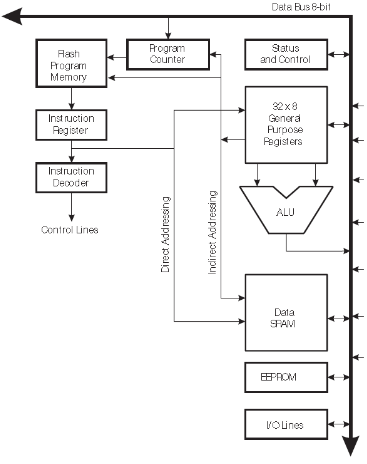
\includegraphics[scale=0.8]{MicroLab1/pictures/1}}
\caption{AVR Architecture}
\end{figure}
CPU Architecture inside. Continuous line, where most of the blocks will be connected, which is called Data Bus 8-bits. The next important block call the Program Memory, it is the type of memory, which is going to restore the programs executing this architecture – Flash memory. The size of this member changes from module to module generally, but we have in our architecture 256KBytes. It is connected to the Data Bus and can exchange data with the rest of modules. After that from this Program memory what we are doing is to obtain the instructions to be executed by the rest of the architecture. Once we get instructions, instruction is in store – in a special register, Instruction Register. It also has a size of memory to load the data, which comes from the Flash memory and then the microcontroller has to decode this instruction. The decoded information will be located in another block Instruction Decoder, which will provide numerous control signals that will be distributed all along the architecture controlling different blocks.\\\\
Another important module is Program Counter or register, which is also connected to the bus, but the most important that it is connected to the Program memory. The Counter block contain the address of the next instruction that will be executed by the microcontroller. The number in
this register is used as an address to go to the program memory and read the instruction, which will be loaded in the Instruction register and then decoded.\\\\
Most of the instructions are going to a temporary store – Register Files. It composed of 32 registers, in each one of them has 8 bits. There is a place where most of the temporary results of the instructions executed by the microcontroller are stored. This block has a connection to the 8-bit Data Bus, but no less important connections is between Registers File and Program Memory. That means that if we want to get some data from the register file and use it as an address to access the program memory. Another important functionality from the register file is to change a value of a Register Counter.\\\\
From the Register File there are additional outputs, to the ALU (Arithmetic Logic Unit). This block is ready to receive to operates, one of them comes from the Register File. By the way, the Register file gets directly the address from the Instruction Register. ALU is performing arithmetical, logical or mathematical operations and writing its values on the data bus.
The Data Memory of type SRAM is implemented to that the program manipulates certain data at its store in this chip. It has a connection to the Data Bus and one connection from the Register File, and connection from the Instruction Register to control the block. From the Register File we can get the data, which can be written in the SRAM memory.\\\\
Status Register is in charge of remembering certain events that occur while instructions are executing in the data path. All the instructions conditions are placed here in 8-bit register and they are stored as a 0 or 1 condition.\\\\
The AVR microcontroller also specialized in I/O operations, it has plenty of the modules that are in charge a performing different I/O operations in all of them are individually connected to the bus. All of them can be controlled also with machine instructions executed within the CPU.
Timers block performs certain tasks related to timers, which is also connected to the bus. ADC comparator, performs a logical task with compare signals. And the last one – Interruptions of microcontroller, it includes interrupts, which can be called within the CPU (Global interrupts, Reset interrupts, Timers interrupts and etc).

\section{Registers}
In a computer, a register is a small amount of storage place that are part of a digital processor. Registers contain a storage address, a computer instruction and so on.
\subsection{General Purpose Register File}
\subsection{XMCRA – External Memory Control Register }
\begin{figure}[H]
\centerline{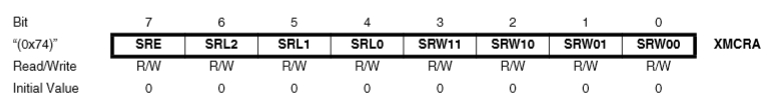
\includegraphics[scale=0.8]{MicroLab1/37last}}
\caption{External Memory Control Register}
\end{figure}
 \paragraph{Bit 7 – SRE: External SRAM/XMEM Enable} SRE controls the External Memory Interface. The value equals one enables the Interface and zero disables.
\paragraph{Bit 6:4 – SRL2:0: Wait-state Sector Limit} External Memory addresses can be configured with different wait-states. It can be done vie dividing of the memory address space into separate wait-state bits. 
\begin{figure}[H]
\caption{Sector limits with different settings of SRL2:0}
\centerline{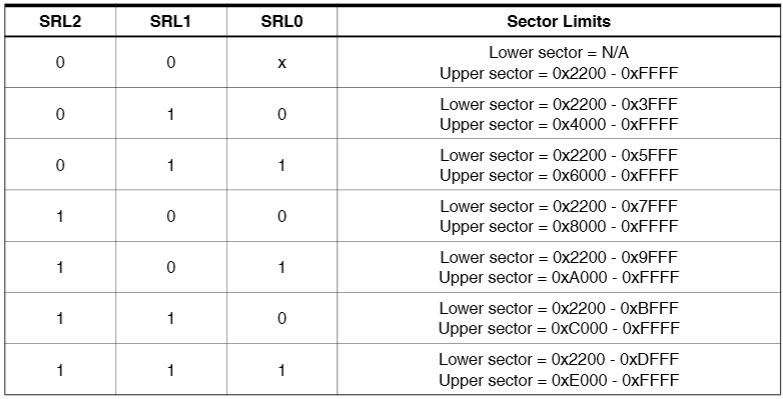
\includegraphics[scale=0.8]{MicroLab1/38p1}}
\end{figure}
\paragraph{Bit 3:2 – SRW11, SRW10: Wait-state Select Bits for Upper Sector} The number of wait-states for the upper sector of the external memory are controlled by the SRW11 and SRW10 bits. 
\paragraph{ Bit 1:0 – SRW01, SRW00: Wait-state Select Bits for Lower Sector}The SRW01 and SRW00 bits do same for lower sector of the address space.
\begin{figure}[H]
\caption{Wait States}
\centerline{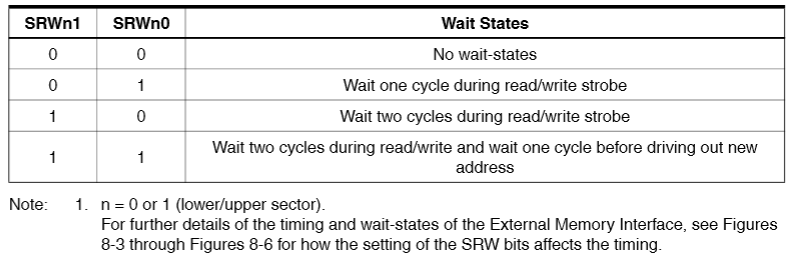
\includegraphics[scale=0.8]{MicroLab1/38p2}}
\end{figure}
\subsubsection{XMCRB – External Memory Control Register B}
\begin{figure}[H]
\centerline{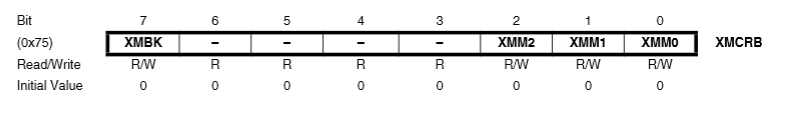
\includegraphics[scale=0.8]{MicroLab1/38p3}}
\caption{External Memory Control Register B}
\end{figure}
\paragraph{Bit 7– XMBK: External Memory Bus-keeper Enable} XMBK values one protects(keeps the last driven value) AD7:0 lines.
\paragraph{Bit 6:3 – Res: Reserved Bits} These bits are reserved future, it must be zero for compatibility with future more modern.
\paragraph{Bit 2:0 – XMM2, XMM1, XMM0: External Memory High} Controls the space of External Memory provided though Port C.
\begin{figure}[h]
\caption{Port C Pins Released as Normal Port Pins when the External Memory is Enabled}
\centerline{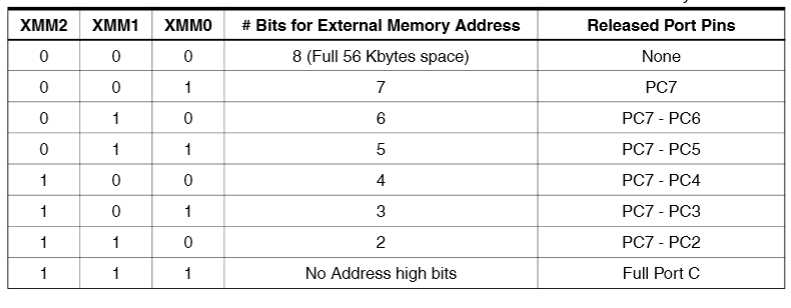
\includegraphics[scale=0.8]{MicroLab1/39p}}
\end{figure}

\subsection{Status registers}
By far the mostly used port is the status register with its 8 bits. Usually access to this port is only by automatic setting and clearing bits by the CPU or accumulator, some access is by reading or branching on certain bits in that port, in a few cases it is possible to manipulate these bits directly (using the assembler command SEx or CLx, where x is the bit abbreviation). Most of these bits are set or cleared by the accumulator through bit-test, compare- or calculation-operations. The following list has all assembler commands that set or clear status bits depending on the result of the execution. 
\begin{figure}[H]
\centerline{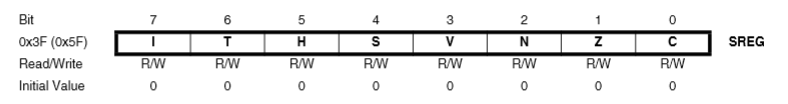
\includegraphics[scale=0.8]{MicroLab1/14p}}
\caption{AVR Status Register}
\end{figure}
The AVR Status Register – SREG – is defined as:

\paragraph{Bit 7 – I: Global Interrupt Enable} The bit controls Global Interrupts. It is possible to turn off all of them by passing zero to the bit.
\paragraph{Bit 6 – T: Bit Copy Storage} There are BLD and BST command. The first one can copy the information from T-bit to a bit in the Register File, the second one can perform the operation in opposite direction.
\paragraph{Bit 5 – H: Half Carry Flag}  a Half Carry indicator for some arithmetic operations.
\paragraph{Bit 4 – S: S-bit} is the Negative FlagN and the Two’s Complement Overflow Flag V an exclusive or. 
\paragraph{Bit 3 – V: Two’s Complement Overflow Flag}  used in two’s complement arthritics. 
\paragraph{Bit 2 – N: Negative Flag} shows a negative result in a logic and an arithmetic operation. 
\paragraph{Bit 1 – Z: Zero Flag}  indicates results of a logic and an arithmetic operation which are equal to zero.
\paragraph{ Bit 0 – C: Carry Flag} indicates a carry in an arithmetic or logic operation. 
\subsection{Stack pointers}
A stack pointer is a small register that stores the address of the last program request in a stack. A stack is a specialized buffer which stores data from the top down. As new requests come in, they "push down" the older ones. The most recently entered request always resides at the top of the stack, and the program always takes requests from the top.\\\\
A stack (also called a pushdown stack) operates in a last-in/first-out sense. When a new data item is entered or "pushed" onto the top of a stack, the stack pointer increments to the next physical memory address, and the new item is copied to that address. When a data item is "pulled" or "popped" from the top of a stack, the item is copied from the address of the stack pointer, and the stack pointer decrements to the next available item at the top of the stack.

\section{Instruction set}
Instructions are the machine commands in machine language, which are obtaining in the CPU by the Program memory (Flash) where the instructions can be executed by the rest of the architecture. Once we get instructions, instruction is in store – in a special register, Instruction Register. It also has a size of memory to load the data, which comes from the Flash memory and then the microcontroller has to decode this instruction. The decoded information will be located in another block Instruction Decoder, which will provide numerous control signals that will be distributed all along the architecture controlling different blocks. The Program Counter or register block, which is also connected to the bus in the CPU, but the most important that it is connected to the Program memory. The Counter block contain the address of the next instruction that will be executed by the microcontroller.\\\\
The list of all instructions we can find on page 416 of the doc2549 manual about Flash Microcontroller programming.
\section{Setting the system clock}

A clock is simply a device that keeps track of time, it kind of gives you a beat to move to. The clock on your wall counts in increments of seconds, for example. A metronome for your instrument might give you a beat every half or full second. The amount of times a clock ticks/cycles per second is called its frequency, measured in Hertz (Hz or cycles/second). Similarly, your ATMega has a clock inside too, and its speed directly relates to how many instructions it can carry out per second (on every tick/cycle of the clock). 
\subsection{Clock Sources}
\begin{figure}[H]
\caption{Device Clocking Options Select}
\centerline{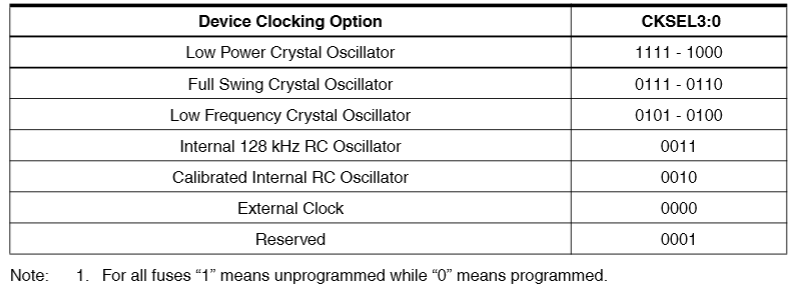
\includegraphics[scale=0.8]{MicroLab1/41p}}
\end{figure}

\subsubsection{Internal RC Oscillator}
This is the default clock source on most AVR microcontrollers. The internal RC Oscillator runs at a frequency of 1MHz by default, but can also be made to run at 2, 4 or 8MHz (speeds depend on the device). Since it is internal, no extra components are needed. The biggest drawback is that the clock frequency varies with the power supply voltage and temperature. Hence, it may not be suitable for applications where a stable clock frequency is needed, such as high speed UART or SPI.
\subsubsection{Crystal/Ceramic Resonator}
These provide a very stable clock signal. They are discrete components that connect to the AVR microcontroller through the XTAL1 and XTAL2 pins. They're usually a bit expensive, but are worth the cost for some applications, especially ones involving synchronous communication. \\\\
Crystals allow the AVR microcontroller to run at various speeds, ranging from a few hundred kHz up to 16MHz; the maximum speed for most devices. 
\subsubsection{External RC Oscillator}
This is formed using a single resistor and capacitor. Accuracy is very poor, and since the AVR microcontroller already has an internal RC oscillator, this option does not seem to make much sense either. The AVR microcontroller can be configured to utilize an internal 36pF capacitor as well, thus needing only an external resistor.


\section{Power management}
When we have an application for embedded system without external power supply, thus energy efficient is very important. The AVR microcontrollers have a several special modes to manage power – Sleep Modes. These modes allows the application to shut down unused modules in the MCU or shut down modules soon after using. For example, Analog-Digital Conversion can be switched off after measurement.
\subsection{Clock Sources}
\begin{figure}[H]
\caption{Sleep Mode Select}
\centerline{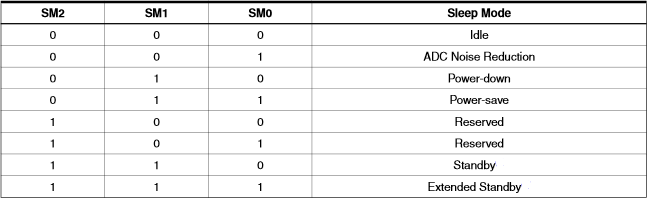
\includegraphics[scale=0.8]{MicroLab1/pictures/2}}
\end{figure}
Sleep modes switch of clocks (CPU clock, Flash memory clock and etc), but stay awake some sources, such as USART, ADC and others. Each mode has its own influence specifications for different parts of microcontroller. If an enabled interrupt occurs while the MCU is in a sleep mode, the MCU wakes up. The MCU is then halted for four cycles in addition to the start-up time, executes the interrupt routine, and resumes execution from the instruction following SLEEP.
\subsection{Idle Mode}
When MCU is in Idle mode by instruction SLEEP, this mode stops the CPU, but allowing he SPI, USART, Analog Comparator, ADC, Timer/Counters and the interrupt system works. It halts only CPUclk and FLASHclk, while allowing the other clocks to run. MCU wakes up from external triggered interrupts as well as internal (Timer Overflow and USART transmit complete) interrupts. To reduce consumption in the Idle mode, the Analog Comparator can be powered down, if it doent required for application.
\subsection{ADC Noise Reduction}
When MCU is in this mode by instruction SLEEP, this mode stops the CPU, but allows the ADC, external interrupts, Timer/Counter2 and Watchdot operating (if enebled). It halts CPUclk and FLASHclk, while others allowed to run. This improves the noise environment for the ADC, it enabling higher resolution measurements. If the ADC is enabled, a conversion starts automatically for this mode. MCU can wake up from the ADC Converion Complete interrupt, an External Reset, a Watchdog System Reset or Interrupt, Timer/Counter2 interrupt and SPM/EEPROM ready interrupt.
\subsection{Power-down Mode}
In this Sleep Mode the external Oscillator is stopped, while interrupts and the 2-wire Serial Interface and the Watchdog operating (if enabled by user). Only External Reset, a Watchdog
Reset, the 2-wire Serial Interface address match, an external level interrupts or a pin change interrupt can wake up the MCU. The MCU can be woken up by a level triggered interrupt, but it will require some time to wake up after the changed level. There is a delay from the wake-up condition occurs until the wake-up becomes effective.
\subsection{Power-Save Mode}
The same as a Power-down Mode, except:\\\\
If Timer/Counter2 is enabled, running happens during sleep. The device can wake up from the Timer Overflow or Output Compare event, if interrupt enable bits on TIMSK2, and the Global Interrupt Enable bit in SREG. If Timer/Counter2 is shut down, the recommended mode is Power-down Mode.
\subsection{Standby Mode}
This mode is identical to Power-down with the exception that the Oscillator is kept running. The device wakes up in six clock cycles in this Standly mode.
\subsection{Extended Standby Mode}
This mode is identical to Power-save mode with the exception that the Oscillator is kept running. The device also wakes up in six clock cycles as in Standby mode.
\section{Resetting the system}
Reset sets all I/O Registers to initial values and the program execution starts from a Reset Vector.
All of I/O ports are resetted to the initial states, clock source does not required.\\\\

There are five sources of reset in the ATmega640/1280/1281/2560/2561:
\begin{itemize}
\item Power-on Reset is performed if the supply voltage is lower than threshold ($V_{POT}$).
\item External Reset is fired by low level of voltage on the RESET pin.
\item Watchdog Reset is fired if it is enabled and the timer period is expired.
\item  Brown-out Reset is performed if the supply voltage VCC is below the Brown-out Reset threshold. Brown-out Detector has to be enabled.
\item  JTAG AVR Reset is fired by high level of voltage on the Reset Register on the JTAG.
\end{itemize}
\section{Memory System}
The AVR architecture has two main memory spaces, the Data Memory and the Program Memory space. In addition EEPROM Memory for data storage. There are three in sum. Program Memory, it is the type of memory, which is going to restore the programs executing this architecture – Flash memory. The size of this member changes from module to module generally, but we have in our architecture 256KBytes. It is connected to the Data Bus in the CPU and can exchange data with the rest of modules.\\\\
The Data Memory of type SRAM is implemented to that the program manipulates certain data at its store in this chip. It has a connection to the Data Bus and one connection from the Register File, which is a place where most of the temporary results of the instructions executed by the microcontroller are stored. That means that if we want to get some data from the register file and use it as an address to access the program memory. From the Register File we can get the data, which can be written in the SRAM memory. There can be also I/O, Extended I/O addresses.
\section{Control Circuit}
\subsection{SPI}
Serial Peripheral Interface or SPI bus is a synchronous serial data link, a de facto standard, named by Motorola, that operates in full duplex mode. It is used for short distance, single master communication, for example in embedded systems, sensors, and SD cards.\\\\
Devices communicate in master/slave mode where the master device initiates the data frame. Multiple slave devices are allowed with individual slave select lines. Sometimes SPI is called a four-wire serial bus, contrasting with three-, two-, and one-wire serial buses. SPI is often referred to as SSI (Synchronous Serial Interface).
\subsection{USART}
A universal asynchronous receiver/transmitter, abbreviated UART, is a piece of computer hardware that translates data between parallel and serial forms. UARTs are commonly used in conjunction with communication standards such as EIA, RS-232, RS-422 or RS-485. The universal designation indicates that the data format and transmission speeds are configurable. The electric signaling levels and methods (such as differential signaling etc.) are handled by a driver circuit external to the UART.\\\\
A UART is usually an individual (or part of an) integrated circuit used for serial communications over a computer or peripheral device serial port. UARTs are now commonly included in microcontrollers. A dual UART, or DUART, combines two UARTs into a single chip. An octal UART or OCTART combines eight UARTs into one package, an example being the NXP SCC2698. Many modern ICs now come with a UART that can also communicate synchronously; these devices are called USARTs (universal synchronous/asynchronous receiver/transmitter).
\subsection{ADC}
An analog-to-digital converter (ADC, A/D, or A to D) is a device that converts a continuous physical quantity (usually voltage) to a digital number that represents the quantity's amplitude.\\\\
The conversion involves quantization of the input, so it necessarily introduces a small amount of error. Instead of doing a single conversion, an ADC often performs the conversions ("samples" the input) periodically. The result is a sequence of digital values that have been converted from a continuous-time and continuous-amplitude analog signal to a discrete-time and discrete-amplitude digital signal.
\subsection{Oscillator Circuits}
An electronic oscillator is an electronic circuit that produces a periodic, oscillating electronic signal, often a sine wave or a square wave. Oscillators convert direct current (DC) from a power supply to an alternating current signal. They are widely used in many electronic devices. \\\\
There is different types of internal oscillators in the circuit and it also possible to get a signal from external ones.
\subsection{JTAG}
Joint Test Action Group (JTAG) is the common name for the IEEE 1149.1 Standard Test Access Port and Boundary-Scan Architecture. It was initially devised by electronic engineers for testing printed circuit boards using boundary scan and is still widely used for this application.\\\\
Today, JTAG is also widely used for IC debug ports. In the embedded processor market, essentially all modern processors implement JTAG when they have enough pins. Embedded systems development relies on debuggers communicating with chips with JTAG to perform operations like single stepping and breakpointing.
\subsection{ISP}
In-system programming (ISP) is the ability of some programmable logic devices, microcontrollers, and other embedded devices to be programmed while installed in a complete system, rather than requiring the chip to be programmed prior to installing it into the system.\\\\
The primary advantage of this feature is that it allows manufacturers of electronic devices to integrate programming and testing into a single production phase, and save money, rather than requiring a separate programming stage prior to assembling the system. This may allow manufacturers to program the chips in their own system's production line instead of buying preprogrammed chips from a manufacturer or distributor, making it feasible to apply code or design changes in the middle of a production run.
\subsection{I/O pins}
The most part of the circuits are connected to the outside world via I/O pins on the board.
\section{AtMega 2560 pins}
I/O ports such as PORTx (where small letter “x” is A, B, C, D, E, F, G, H, J, K or L) are 8-bit bi-directional I/O ports with internal pull-up resistors (selected for each bit). Each of these ports serves the functions of special features of the Atmega2560. Each of them has their special propose, which make them unique: PORTB has better driving capabilities than others ports, or PORTF serves as analog inputs to the A/D Converter. It also serves the functions of the JTAG interface. If the JTAG interface is enables, the pull-up resistors on pins PF7 (TDI), PF5 (TMS) and PF4 (TCK) will be activated even if a reset occurs.
\subsection{Clock Sources}
\begin{figure}[H]
\caption{Alternate Port Functions}
\centerline{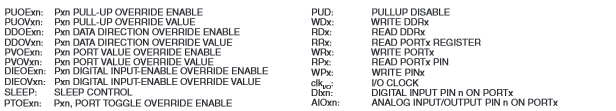
\includegraphics[scale=0.8]{MicroLab1/pictures/3}}
\end{figure}
Because of most of the ports look the same, we can discuss about some of the most interesting PORTs for us, explained below, because of their feature for programming. All the pins call the Change Pin interrupt and pins can serve as an external interrupt source, for example to wake up the MCU from the Sleep Mode. Each of them has Timer/Counterx or Output Compare from Px7-Px4, then for example in PORTD there is the most interesting alternative function, answering for interrupts of the USART Transceiver and Receiver, see below:
\subsection{PORTD}
NT3/TXD1 – Port D, Bit 3. INT3, External Interrupt source 3: The PD3 pin can serve as an external interrupt source to the MCU. TXD1, Transmit Data (Data output pin for the USART1). When the USART1 Transmitter is enabled, this pin is configured as an output regardless of the value of DDD3.\\\\
INT2/RXD1 – Port D, Bit 2. INT2, External Interrupt source 2. The PD2 pin can serve as an External Interrupt source to the MCU. RXD1, Receive Data (Data input pin for the USART1). When the USART1 receiver is enabled this pin is configured as an input regardless of the value of DDD2. When the USART forces this pin to be an input, the pull-up can still be controlled by the PORTD2 bit.
\subsection{PORTE}
AIN1/OC3A – Port E, Bit 3. AIN1 – Analog Comparator Negative input. This pin is directly connected to the negative input of the Analog Comparator.\\\\
AIN0/XCK0 – Port E, Bit 2. AIN0 – Analog Comparator Positive input. This pin is directly connected to the positive input of the Analog Comparator.\\\\
Negative and Positive voltages in A/D converter of the AVR used for differential conversion.
\subsection{PORTF}
This port has an alternate function as analog input for the ADC (PF0-PF3) and enabling JTAG debugging interfaces on pins (PF4-PF7).
\begin{figure}[H]
\caption{Port F pins Alternate Functions}
\centerline{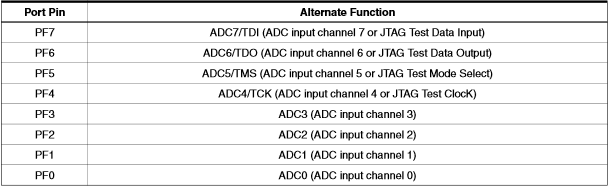
\includegraphics[scale=0.8]{MicroLab1/pictures/4}}
\end{figure}
\subsection{PORTK}
Some ports like Port K are used for Analog-to-Digital Conversations (PK0-PK7) occurs (ADC8-ADC15). Others ports looks the same between each other, the difference between them, that they have another numeric number of a Timer/Counter/External Interrupt (from 0-5) on pins 0,1, 4, 6, 7.\\\\
Example: PORT D
\begin{figure}[H]
\caption{Port D pins Alternate Functions}
\centerline{
\includegraphics[scale=0.8]{MicroLab1/pictures/5}}
\end{figure}
T0 – Port D, Bit 7. T0, Timer/Counter0 counter source.\\\\
T1 – Port D, Bit 6. T1, Timer/Counter1 counter source.\\\\
XCK1 – Port D, Bit 5. XCK1, USART1 External clock. The Data Direction Register (DDD5) controls whether the clock is output (DDD5 set) or input (DDD5 cleared). The XCK1 pin is active only when the USART1 operates in Synchronous mode.\\\\
ICP1 – Port D, Bit 4. ICP1 – Input Capture Pin 1: The PD4 pin can act as an input capture pin or Timer/Counter1.\\\\
INT0/SCL – Port D, Bit 0. INT0, External Interrupt source 0. The PD0 pin can serve as an external interrupt source to the MCU.\\\\
How to set signals for Alternate Functions to the PORTx pins see (8-bit Microcontroller with 256K Bytes In-System Programmable Flash Atmega2560) manual p.78-95.\\\\
VCC – is the digital supply voltage for processor.\\\\
AVCC – is the supply voltage pin for PORTF and the A/D Converter, which is externally connected to VCC, even if the ADC is not used. If the ADC is used, it should be connected to VCC through a low-pass filter.\\\\
AREF – is the analog reference pin for the A/D Converter. Can be configured in the application for different types of ADC conversions.\\\\
GND – Ground.\\\\
XTAL1 and XTAL2 are the input and output the inverting Oscillator amplifier. XTAL1 also is input to the internal clock operating circuit.\\\\
RESET – is the reset input.
\end{document}
